\section{Comparison of all pretrained CV Models}
\label{sxn:all_cv_models}


Here, we use the Weightwatcher tool to analyze 466 pretrained computer vision models Pytorch. These image classification and segmentation models are pretrained on nine datasets, ImageNet-1K, and CIFAR-10, CIFAR-100, Street View House Numbers (SVHN), Caltech-UCSD Birds-200-2011 (CUB-200-2011), Pascal VOC2012, ADE20K, Cityscapes, and Common Objects in Context (COCO). The pretrained models and their accuracy metrics are summarized in the osmr github 


\charlesx{We actually don't run regressions on all these datasetsm, BUT we could present them in the Figure below to show that alpha is a good metric for these kinds of models, in contrast to the NLP, where alpha is frequently too large to run a regression}

\begin{figure}[t]
    \centering
    \subfigure[ImageNet 1K]{
        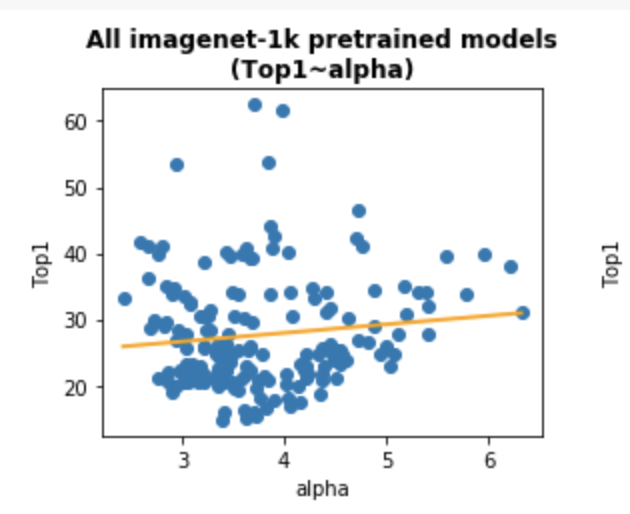
\includegraphics[width=4cm]{img/imagenet1k_alpha.png}
        \label{fig:imagenet1k-alpha}
    }
    \qquad
    \subfigure[ CIFAR 10 ]{
        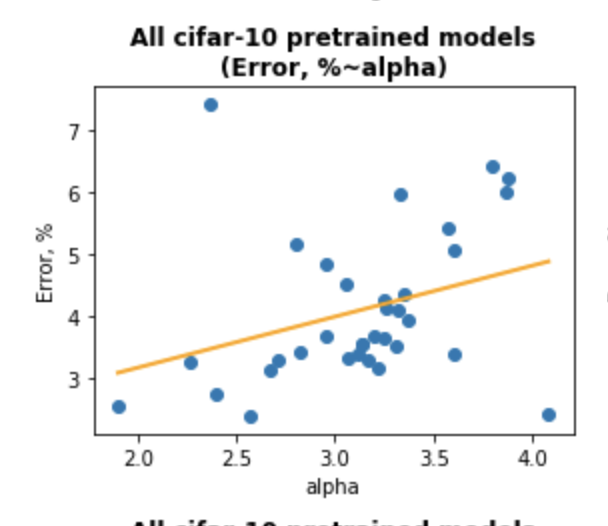
\includegraphics[width=4cm]{img/cifar10_alpha.png}
        \label{fig:cifar10.alpha}
    }
    \qquad
    \subfigure[ CIFAR 100 ]{
        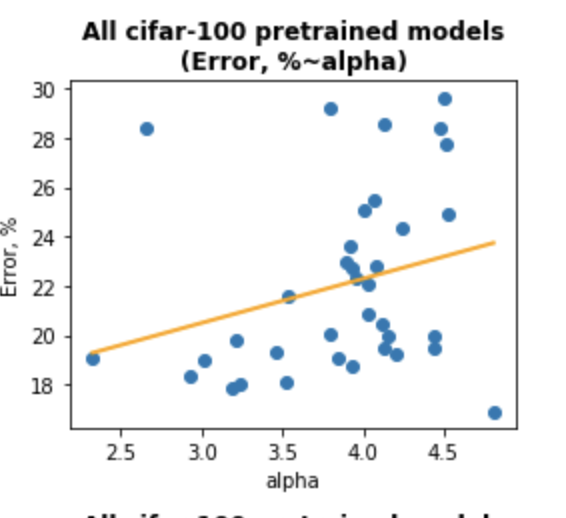
\includegraphics[width=4cm]{img/cifar100_alpha.png}
        \label{fig:cifar100.alpha}
    }
    \qquad
    \subfigure[ SVHN ]{
        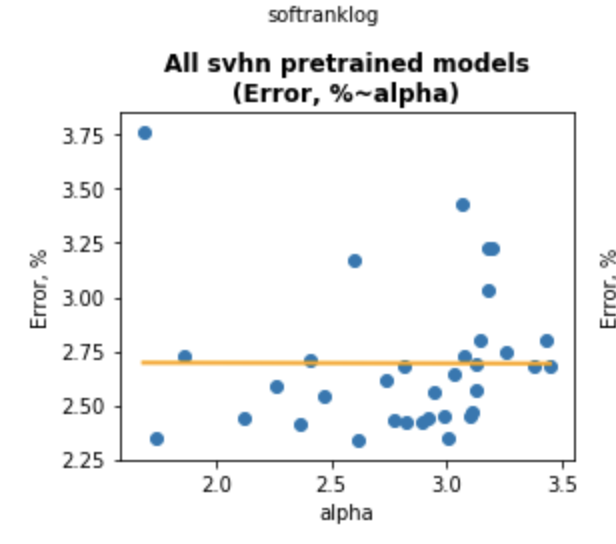
\includegraphics[width=4cm]{img/svhn_alpha.png}
        \label{fig:svhn.alpha}
    }
    \qquad
    \subfigure[ CUB 200 ]{
        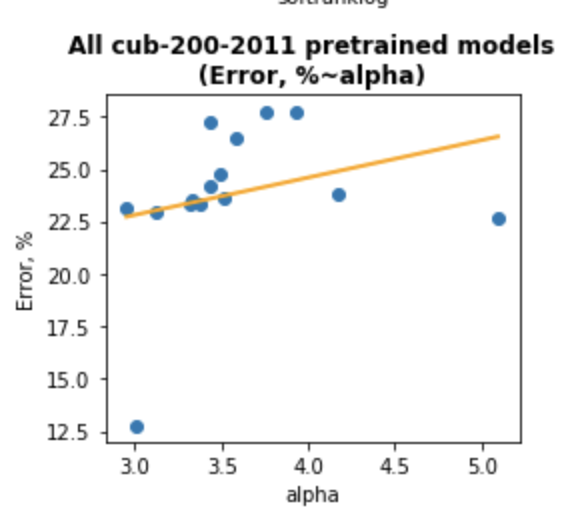
\includegraphics[width=4cm]{img/cub200_alpha.png}
        \label{fig:cub200.alpha}
    }
    \caption{\charles{Preliminary charts:} Heavy Tailed Power Law exponent $\alpha$ vs. reported Top1 Test Accuracies for pretrained DNNs available\charles{ref} for 5 different data sets.}

    \label{fig:dataset_alphas}
\end{figure}




\serena{insert link in the footnote}

and a full summary of all the models analyzed is included in the Appendix. For our analysis, we then group models by architecture and datasets for further analysis.

In this paper, we propose that the Weightwatcher tool could be used to predict the trends in the generalization accuracy of deep neutral network without a test set. To test our proposition, we choose simple linear regression to analyze the relationship between the Weightwatcher metrics and the traditional accuracy metric obtained with a test set (we avoid polynomial regressions as they are more prone to overfitting and does not make economic sense). On the left-hand-side of regression, we have the Top1 errors, Top5 errors as reported for ImageNet-1K models, Error % as reported in CIFAR-10/100, SVHN, CUB-200-2011 models, and Pixel accuracy (Pix.Acc.,%) and Intersection-Over-Union (mIOU,%) as dependent variables. We then regress them individually on each of the Weightwatcher metrics, including  alpha, alpha_weighted, spectralnormlog, softranklog, lognorm, and logpnorm as defined in earlier section. 

\serena{Question: only the alpha-related metrics is the core metrics of the WW tool, right? Metrics such as stable rank or spectral norm have been suggested in other paper before???}

\serena{insert a simple formula for linear regression}

To further refine our analysis, we run three batches of linear regressions. First at the global level, we divide models by datasets and run regression separately on all models of a certain dataset, regardless of the architecture. At this level, the plots are quite noisy and clustered as each architecture has its own accuracy trend but, you could still see that most plots show positive relationship with positive coefficients

\serena{see examples in Figure X}

(Here we omit the results for CUB-200-2011, Pascal-VOC2012, ADE20K, and COCO datasets as there are less than 15 models for those datasets and thus the regression is less statistically significant)

\serena{insert plots for Figure X}

For the second batch, we plot the regression for models of each architecture-datasets combination, which shows the relationship between the progression of the model accuracy and Weightwatcher metrics more clearly and precisely. For example, as you could see in the Figure X2, 

\serena{Add an example, UPDATE when we have the results from the new codes}

Insert plots for Figure X2

While running each regression, we record the R-squared and mean squared errors (MSE) for each regression. We then filter out regressions with less than five datapoints and models with structural outliers.

\serena{Define and give an example of the structural outliers}

\charles{What are the structrual outliers we chose ?}

Insert a plot for outliers, OPTIONAL

\charles{These tables could go to appendix. We need references}

\begin{table}[t]
\small
\begin{center}
\begin{tabular}{|p{1in}|c|}
\hline
Dataset & $\#$ of Models \\
\hline
imagenet-1k   &  78 \\
svhn          &  30 \\
cifar-100     &  30 \\
cifar-10      &  18 \\
cub-200-2011  &  12 \\
\hline
\end{tabular}
\end{center}
\caption{Datasets used}
\label{table:datasets}
\end{table}




\begin{table}[t]
\small
\begin{center}
\begin{tabular}{|p{3in}|c|}
\hline
Architecture & $\#$ of Models \\
\hline
ResNet                                     & 30 \\
SENet/SE-ResNet/SE-PreResNet/SE-ResNeXt    & 24 \\
DIA-ResNet/DIA-PreResNet                   & 18 \\
ResNeXt                                    & 12 \\
WRN                                        & 12 \\
DLA                                        & 6 \\
PreResNet                                  & 6 \\
ProxylessNAS                               & 6 \\
VGG/BN-VGG                                 & 6 \\
IGCV3                                      & 6 \\
EfficientNet                               & 6 \\
SqueezeNext/SqNxt                          & 6 \\
ShuffleNet                                 & 6 \\
DRN-C/DRN-D                                & 6 \\
ESPNetv2                                   & 6 \\
HRNet                                      & 6 \\
SqueezeNet/SqueezeResNet                   & 6 \\
\hline
\end{tabular}
\end{center}
\caption{Architectures used}
\label{table:architectures}
\end{table}




\charles{Still preliminary, only 309 data points here}
\paragraph{Results}
\begin{table}[t]
\small
\begin{center}
\begin{tabular}{|p{1in}|c|c|c|c|}
\hline
    & Frobenius Norm & Spectral Norm & Weighted Alpha & Alpha-Norm \\
    & $\langle\log\Vert\mathbf{W}\Vert_{F}\rangle$ & $\langle\log\Vert\mathbf{W}\Vert_{\infty}\rangle$ & $\langle\hat{\alpha}=\alpha\log\lambda_{max}\rangle$ & $\langle\log\Vert\mathbf{X}\Vert^{\alpha}_{\alpha}\rangle$ \\
\hline
$R^{2}$ (mean) & 0.63 &0.55 &0.64 &0.64 \\
$R^{2}$ (std)  & 0.34 &0.36 &0.29 &0.30 \\
\hline
$MSE$ (mean)   & 4.54 &9.62 &3.14 &2.92 \\
$MSE$ (std)    & 8.69 &23.06 &5.14 &5.00 \\
\hline
\end{tabular}
\end{center}
\caption{Comparison of linear regression fits for different average log norm metrics across 5 computer vision datasets, 17 Architectures, covering 168 (out of 309) different pretrained DNNs.  We only conclude regressions for architecturs with 4 or more data points \charles{and which are postively correlated with the test error?}.  These results can be readily reproduced using the Google Colab notebooks accompanying thie paper\cite{notebooks}}
\label{table:results}
\end{table}


